\chapter{From Particles to a Simple Quantum Field}

Let us build the simple quantum field once more, but from a slightly different angle. There are two roads into quantum field theory. We may begin with particles and discover why a field is the natural language for them, or begin with a wave field and discover why its excitations come in quanta. Both roads are useful. Here we stay on the first one.

Ordinary quantum mechanics can describe one particle, two particles, or any other fixed number. Nature does not respect that restriction. The number of photons in a room changes whenever the lights emit or absorb radiation. Unstable particles decay. In beta decay, for example,
\begin{equation}
n\longrightarrow p+e^-+\bar{\nu}_e,
\end{equation}
so the populations of several particle species change at once. We therefore want one quantum mechanics large enough to contain every possible occupation number and, eventually, processes that move among them.

For the moment we simplify severely. There is one species of nonrelativistic particle. We shall first enlarge its state space so that it can hold any particle number, and only afterward discuss more species, relativity, scattering, and decay. None of the mathematics is especially hard, but the change of viewpoint is abstract. It is worth taking the steps slowly enough that the notation does not hide the idea.

\section{The One-Particle Starting Point}

Begin with a single particle in a state \(|\psi\rangle\). Its position-space wavefunction is
\begin{equation}
\psi(x)=\langle x|\psi\rangle.
\label{eq:l07-wavefunction}
\end{equation}
This lower-case \(\psi\) is an ordinary complex-valued function. It is not yet a quantum field and it is not an operator on a many-particle state space.

The Born rule says that
\begin{equation}
\rho_\psi(x)=|\psi(x)|^2=\psi^*(x)\psi(x)
\label{eq:l07-born-density}
\end{equation}
is the probability density for finding the particle at \(x\). For a normalized state,
\begin{equation}
\int dx\,\psi^*(x)\psi(x)=1.
\label{eq:l07-one-particle-normalization}
\end{equation}
The right-hand side is the total probability. Since this problem contains exactly one particle, it also happens to equal the number of particles. That coincidence will become a useful clue, although it is trivial here.

\begin{classroomqa}
\lecturetimestamp{00:09:13}
\audiencequestion{Why must the probability density have the form \(\psi^*(x)\psi(x)\)?}
\lecturerresponse{That is the Born rule, one of the postulates of quantum mechanics. The amplitude for the position outcome \(x\) is \(\langle x|\psi\rangle\); the probability density is its absolute square. It is not derived from the field construction used later.}
\end{classroomqa}

\section{Modes, Orthogonality, and Completeness}

There are many useful bases for the one-particle Hilbert space. Position eigenstates form one basis. The eigenstates of any Hermitian operator form another, with the usual qualifications for degeneracies and continuous spectra. Since energy will soon matter, choose a complete orthonormal set of one-particle energy eigenstates
\begin{equation}
|1\rangle,\ |2\rangle,\ldots,
\qquad
\psi_i(x)=\langle x|i\rangle.
\end{equation}

A particle in a box makes the index \(i\) concrete. The ground-state wavefunction has no interior node, the next state has one, and the higher states oscillate more rapidly. They are essentially sine waves for an ideal infinite square well.

\begin{figure}[htbp]
\centering
\includegraphics[width=0.94\linewidth]{lecture_07_frame_01.png}
\caption{The box modes on the lecture board. The remnants at left are the one-particle Born density and normalization; the well at right shows \(\psi_1(x)\), \(\psi_2(x)\), and the general label \(\psi_i(x)\).}
\lectureframe{00:08:25}
\end{figure}

The same mode structure can be separated from the live-board occlusion:
\begin{figure}[htbp]
\centering
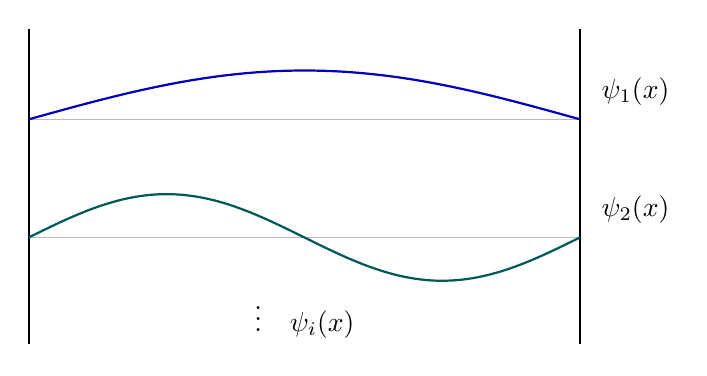
\begin{tikzpicture}[x=1cm,y=1cm]
  \draw[thick] (0,0) -- (0,4.0);
  \draw[thick] (7,0) -- (7,4.0);
  \draw[gray!55] (0,2.85) -- (7,2.85);
  \draw[gray!55] (0,1.35) -- (7,1.35);
  \draw[blue!75!black,thick,domain=0:7,samples=120]
    plot (\x,{2.85+0.62*sin(180*\x/7)});
  \draw[teal!70!black,thick,domain=0:7,samples=120]
    plot (\x,{1.35+0.55*sin(360*\x/7)});
  \node[right] at (7.15,3.20) {$\psi_1(x)$};
  \node[right] at (7.15,1.70) {$\psi_2(x)$};
  \node at (3.5,0.38) {$\vdots\quad\psi_i(x)$};
\end{tikzpicture}
\caption{A clean reconstruction of the qualitative box sketch. The vertical offsets merely separate the two wavefunctions for display.}
\end{figure}

Orthonormality is
\begin{equation}
\int dx\,\psi_i^*(x)\psi_j(x)=\delta_{ij}.
\label{eq:l07-orthonormality}
\end{equation}
If \(i=j\), the state is normalized and the integral is one. If \(i\ne j\), the two states are orthogonal and the integral vanishes.

Completeness is the equally important statement
\begin{equation}
\sum_i |i\rangle\langle i|=\mathbf 1.
\label{eq:l07-resolution}
\end{equation}
Each \(|i\rangle\langle i|\) projects onto one basis direction; the sum over the complete basis is the identity. Acting on an arbitrary vector merely decomposes that vector into its components and puts it back together.

Now sandwich Equation~\eqref{eq:l07-resolution} between two position states:
\begin{align}
\langle y|x\rangle
&=\sum_i\langle y|i\rangle\langle i|x\rangle \\
&=\sum_i\psi_i(y)\psi_i^*(x) \\
&=\delta(y-x).
\label{eq:l07-position-completeness}
\end{align}
The star belongs on the factor whose bra-ket order is \(\langle i|x\rangle\). Reversing \(x\) and \(y\) gives the complex-conjugate but equivalent form. Thus every complete orthonormal basis supplies a representation of the delta function. Sines, cosines, oscillator wavefunctions, and energy eigenfunctions all do the same job.

\begin{classroomqa}
\lecturetimestamp{00:13:43}
\audiencequestion{Should the second wavefunction in the completeness sum carry the complex conjugate?}
\lecturerresponse{Yes. With the order \(\langle y|i\rangle\langle i|x\rangle\), the factors are \(\psi_i(y)\psi_i^*(x)\). Keeping the bra-ket order visible prevents the star from being guessed or misplaced.}
\end{classroomqa}

This is the one-particle mathematics we shall need. We now change the state space.

\section{Fock Space as the Larger State Space}

For many identical particles, a convenient basis records how many particles occupy each one-particle mode:
\begin{equation}
|n_1,n_2,n_3,\ldots\rangle.
\label{eq:l07-fock-basis}
\end{equation}
The integer \(n_i\) is the occupation number of mode \(i\). This ket is not a one-particle state written in fancy notation. It belongs to a larger Hilbert space containing the zero-particle sector, every one-particle state, every two-particle state, and so on. That larger space is called Fock space.

To change occupations, introduce for every mode a creation operator and an annihilation operator,
\begin{equation}
a_i^\dagger,\qquad a_i.
\end{equation}
The first adds one particle to mode \(i\), while the second removes one. At this stage the harmonic-oscillator language is a bookkeeping device: there need not be a literal spring oscillating. The oscillator algebra gives us exactly the machinery needed to raise and lower occupation numbers.

The mode number operator is
\begin{equation}
\begin{aligned}
N_i&=a_i^\dagger a_i,\\
N_i|n_1,\ldots,n_i,\ldots\rangle
&=n_i|n_1,\ldots,n_i,\ldots\rangle.
\end{aligned}
\end{equation}
The vacuum is
\begin{equation}
|0\rangle\equiv|0,0,0,\ldots\rangle,
\qquad
a_i|0\rangle=0
\quad\text{for every }i.
\label{eq:l07-vacuum}
\end{equation}
A one-particle state in mode \(i\) is therefore
\begin{equation}
|i\rangle=a_i^\dagger|0\rangle.
\label{eq:l07-mode-created}
\end{equation}
The same symbol \(|i\rangle\) can now be read either as a one-particle basis vector or as that vector embedded in the one-particle sector of Fock space. The embedding is Equation~\eqref{eq:l07-mode-created}; the surrounding context tells us which space is being discussed.

\section{Packaging the Modes into a Field}

Define the annihilation and creation fields by
\begin{equation}
\Psi(x)=\sum_i \psi_i(x)a_i,
\qquad
\Psi^\dagger(x)=\sum_i \psi_i^*(x)a_i^\dagger.
\label{eq:l07-field-expansion}
\end{equation}
The capital letter matters. The lower-case functions \(\psi_i(x)\) are complex numbers; the capital \(\Psi(x)\) is an operator on Fock space. At every spatial point \(x\), Equation~\eqref{eq:l07-field-expansion} gives a different linear combination of the mode operators. That is what an operator-valued function of position means.

For free particles the mode functions may be plane waves \(e^{ikx}\). Then Equation~\eqref{eq:l07-field-expansion} is a Fourier expansion, except that its Fourier coefficients are operators rather than numbers. The old terminology calls ordinary complex numbers \(c\)-numbers and quantum operators \(q\)-numbers. The mode functions are \(c\)-numbers and commute with everything; the \(a_i\) and \(a_i^\dagger\) carry the operator character.

Neither \(\Psi\) nor \(\Psi^\dagger\) is Hermitian. Their adjoints are each other. The two combinations
\begin{equation}
\Psi+\Psi^\dagger,
\qquad
i(\Psi^\dagger-\Psi)
\label{eq:l07-hermitian-combinations}
\end{equation}
are Hermitian and can represent observables. For the moment, however, the fields are most useful as devices that create, annihilate, and count particles locally.

\begin{classroomqa}
\lecturetimestamp{00:21:05}
\audiencequestion{What does it mean for an operator to depend on \(x\)?}
\lecturerresponse{It means that each value of \(x\) selects a different operator. The spatial dependence sits in the ordinary mode functions, while each resulting linear combination acts on the same Fock space.}
\end{classroomqa}

\section{What the Creation Field Does}

A definition becomes useful when we ask what it does. Start with a position eigenstate in the one-particle sector and insert the resolution of identity:
\begin{align}
|x\rangle
&=\sum_i |i\rangle\langle i|x\rangle \\
&=\sum_i a_i^\dagger|0\rangle\,\psi_i^*(x) \\
&=\Psi^\dagger(x)|0\rangle.
\label{eq:l07-local-creation}
\end{align}
Thus \(a_i^\dagger\) creates a particle in the definite mode \(i\), whereas \(\Psi^\dagger(x)\) creates a particle localized at \(x\). In the idealized position basis that localization is distributional; a physical preparation would use a narrow wavepacket, but the algebraic meaning is the same.

\begin{classroomqa}
\lecturetimestamp{00:24:48}
\audiencequestion{Is \(\sum_i|i\rangle\langle i|\) a projection?}
\lecturerresponse{Each term is a projection onto one basis state. The complete sum is the identity itself and is called a resolution of the identity. Inserting it changes no state, but exposes the state's components in the chosen basis.}
\end{classroomqa}

Equation~\eqref{eq:l07-local-creation} is the first direct particle interpretation of the field. We have not merely attached a spatial label to an abstract operator. We have built the operation that makes a particle at that spatial point.

\begin{classroomqa}
\lecturetimestamp{00:28:20}
\audiencequestion{Should the position-space creation field be marked with a star or a dagger?}
\lecturerresponse{Use a dagger for an operator adjoint. Stars denote complex conjugation of the ordinary wavefunctions \(\psi_i(x)\); daggers belong on \(a_i^\dagger\) and \(\Psi^\dagger(x)\).}
\end{classroomqa}

\begin{classroomqa}
\lecturetimestamp{00:28:36}
\audiencequestion{May the creation operators be moved past the wavefunctions in the mode expansion?}
\lecturerresponse{Yes. The \(\psi_i(x)\) are \(c\)-numbers, so they commute with every operator. One must be careful only when changing the order of noncommuting operators such as \(a_i\) and \(a_j^\dagger\).}
\end{classroomqa}

\section{From Probability Density to Particle Density}

Let us now play with the field. The first natural expression is
\begin{equation}
\int dx\,\Psi^\dagger(x)\Psi(x).
\end{equation}
It looks like the one-particle normalization integral, but its factors are now operators. Insert the mode expansions without changing their order:
\begin{align}
\int dx\,\Psi^\dagger(x)\Psi(x)
&=\int dx
\left(\sum_i a_i^\dagger\psi_i^*(x)\right)\\
&\qquad\times\left(\sum_j a_j\psi_j(x)\right) \\
&=\sum_{i,j}a_i^\dagger a_j
\int dx\,\psi_i^*(x)\psi_j(x) \\
&=\sum_{i,j}a_i^\dagger a_j\,\delta_{ij} \\
&=\sum_i a_i^\dagger a_i.
\label{eq:l07-number-derivation}
\end{align}
Hence the total-number operator is
\begin{equation}
N=\sum_i N_i
=\int dx\,\Psi^\dagger(x)\Psi(x).
\label{eq:l07-total-number}
\end{equation}
For the states under discussion, finite-energy excitations have occupations that die away at sufficiently high mode energy, so this total is ordinarily finite even though the list of possible modes is infinite.

The integrand is the local particle-density operator:
\begin{equation}
n(x)=\Psi^\dagger(x)\Psi(x).
\label{eq:l07-density}
\end{equation}
Strictly speaking one does not measure the density at a mathematical point. For a small region \(R\), one measures
\begin{equation}
N_R=\int_R dx\,n(x),
\label{eq:l07-regional-number}
\end{equation}
the number of particles in that region. Like any quantum observable, \(N_R\) need not have a definite value in an arbitrary state. Repeated preparations can yield different outcomes.

\begin{classroomqa}
\lecturetimestamp{00:36:27}
\audiencequestion{Is \(\Psi^\dagger(x)\Psi(x)\) the many-particle probability density?}
\lecturerresponse{Its direct meaning is particle density. A many-particle probability amplitude generally depends on all particle coordinates. The local bilinear instead counts particles in a small region when integrated over that region.}
\end{classroomqa}

\begin{classroomqa}
\lecturetimestamp{00:38:28}
\audiencequestion{Do the operators \(a_i\) and \(a_i^\dagger\) act only on state vectors and not on the one-particle wavefunctions?}
\lecturerresponse{Yes. They act on Fock-space states such as \(|n_1,n_2,\ldots\rangle\). The one-particle mode functions multiplying them are ordinary numbers and are not the objects on which these ladder operators act.}
\end{classroomqa}

The occupation kets form a basis, not the most general state. They may be superposed, including superpositions in which the same total number is distributed differently among the modes. For neutral species such as photons, one may also superpose different total particle numbers. The operator in Equation~\eqref{eq:l07-regional-number} retains the same operational meaning in every such state.

\begin{classroomqa}
\lecturetimestamp{00:40:01}
\audiencequestion{If the particle density is divided by the total number, does it become the probability density for finding a particle at \(x\)?}
\lecturerresponse{In a fixed-\(N\), large-population setting, \(N_R/N\) is a relative frequency and usually tracks a one-particle probability very well. It is not an operator identity equating one measurement outcome with a probability. The measured count fluctuates, typically by an amount of order \(\sqrt N\) in an independent-particle picture, and an exceptional run can differ greatly from the probability even though such a run is unlikely.}
\end{classroomqa}

\begin{classroomqa}
\lecturetimestamp{00:42:25}
\audiencequestion{What happens to charge conservation in a superposition of a one-electron state and a zero-electron state?}
\lecturerresponse{That is not the kind of superposition used for a closed sector of fixed electric charge. One may superpose different distributions with the same total charge. Photons carry no electric charge, so different photon-number sectors cause no such problem. Electron and positron numbers may also change together while the net charge remains fixed.}
\end{classroomqa}

\section{The Energy of Independent Particles}

The next observable is energy. Restrict first to particles that do not interact with one another. This is often a good approximation in a dilute system. Even photons interact in principle through higher-order processes, but ordinary laboratory radiation is dilute enough that the independent-particle description is excellent.

Let \(\omega_i\) denote the energy of one particle in mode \(i\), with \(\hbar=1\). A mode means one one-particle state. The total Hamiltonian is then
\begin{equation}
H=\sum_i\omega_i N_i
=\sum_i\omega_i a_i^\dagger a_i.
\label{eq:l07-mode-hamiltonian}
\end{equation}
Each occupied mode contributes its one-particle energy once per particle.

\begin{classroomqa}
\lecturetimestamp{00:48:16}
\audiencequestion{Is \(\omega_i\) a function of position?}
\lecturerresponse{No. It is the energy eigenvalue associated with mode \(i\). The function \(\psi_i(x)\) depends on position; \(\omega_i\) depends on which energy level has been selected.}
\end{classroomqa}

The values \(\omega_i\) are determined by the one-particle time-independent Schrodinger equation. Define
\begin{equation}
h=-\frac{\nabla^2}{2m}+V(x).
\label{eq:l07-one-particle-h}
\end{equation}
Then
\begin{equation}
h\psi_i(x)=\omega_i\psi_i(x).
\label{eq:l07-schrodinger-eigenvalue}
\end{equation}
In one dimension the momentum operator is \(p=-i\partial_x\), and \(p^2/(2m)\) becomes \(-\partial_x^2/(2m)\). In three dimensions the three second derivatives combine into \(-\nabla^2/(2m)\).

\begin{figure}[htbp]
\centering
\includegraphics[width=0.94\linewidth]{lecture_07_frame_02.png}
\caption{The board passage from \(p^2/(2m)+V(x)\) to the differential form of the one-particle Schrodinger eigenvalue equation. Equation~\eqref{eq:l07-schrodinger-eigenvalue} is its cleaned reconstruction.}
\lectureframe{00:54:10}
\end{figure}

For an arbitrary normalized one-particle wavefunction, the familiar expectation value is
\begin{equation}
\langle h\rangle_\psi
=\int dx\,\psi^*(x)h\psi(x).
\label{eq:l07-one-particle-energy-expectation}
\end{equation}
The many-particle formula is suggested by replacing the lower-case wavefunction with the operator-valued field. This is not yet a proof; it is the guess whose correctness we now test:
\begin{equation}
H=\int dx\,\Psi^\dagger(x)h\Psi(x).
\label{eq:l07-field-hamiltonian}
\end{equation}

\section{Writing the Answer First, Then Proving It}

Insert Equation~\eqref{eq:l07-field-expansion} into the proposed Hamiltonian:
\begin{align}
\int dx\,\Psi^\dagger h\Psi
&=\int dx
\left(\sum_i a_i^\dagger\psi_i^*(x)\right)
h\left(\sum_j a_j\psi_j(x)\right) \\
&=\sum_{i,j}a_i^\dagger a_j
\int dx\,\psi_i^*(x)h\psi_j(x).
\label{eq:l07-h-expanded}
\end{align}
The differential operator \(h\) acts on the \(x\)-dependent wavefunction \(\psi_j(x)\), not on the mode operator \(a_j\). By the Schrodinger equation,
\begin{equation}
h\psi_j(x)=\omega_j\psi_j(x).
\end{equation}
Consequently,
\begin{align}
\int dx\,\Psi^\dagger h\Psi
&=\sum_{i,j}a_i^\dagger a_j\omega_j
\int dx\,\psi_i^*(x)\psi_j(x) \\
&=\sum_{i,j}a_i^\dagger a_j\omega_j\delta_{ij} \\
&=\sum_j\omega_j a_j^\dagger a_j.
\label{eq:l07-h-proof}
\end{align}
This is precisely Equation~\eqref{eq:l07-mode-hamiltonian}. The local field expression and the sum of all particle energies are the same operator.

\begin{figure}[htbp]
\centering

\includegraphics[width=0.94\linewidth]{lecture_07_frame_03.png}
\caption{The field Hamiltonian emphasized on the board, with the mode-expansion proof beginning below it. The live frame is retained as evidence; Equations~\eqref{eq:l07-field-hamiltonian}--\eqref{eq:l07-h-proof} restore the complete algebra.}
\lectureframe{01:05:34}
\end{figure}

No creation operator has been commuted past an annihilation operator in this derivation. The \(a_i^\dagger a_j\) order is maintained from beginning to end. The only freely moved objects are the \(c\)-number wavefunctions and their eigenvalues.

\section{Why This Is a Field}

Why call \(\Psi(x)\) a field? Because it is an operator-valued quantity defined at every point of space, and Hermitian combinations or bilinears constructed from it are local observables. The density \(n(x)\) and the local energy expression below are two examples. There is no additional mathematical test hidden behind the word.

This field is not the electromagnetic field. It describes whichever nonrelativistic species supplied the one-particle modes and the Hamiltonian \(p^2/(2m)+V\): slowly moving atoms, neutrons, protons, or electrons, for example. Those particles are the quanta of their corresponding field, in the same structural sense that photons are the quanta of the electromagnetic field.

\begin{classroomqa}
\lecturetimestamp{01:02:45}
\audiencequestion{Where, in passing from the many-particle system to the formula above, did a field enter?}
\lecturerresponse{It entered in Equation~\eqref{eq:l07-field-expansion}: \(\Psi(x)\) is an operator at every spatial point. The subsequent derivations show that its local products measure particle and energy densities. Position dependence plus operator content is exactly the field structure being constructed.}
\end{classroomqa}

\section{Local Energy Density}

Equation~\eqref{eq:l07-field-hamiltonian} writes the total energy as an integral over space,
\begin{equation}
\begin{aligned}
H&=\int dx\,\mathcal H(x),\\
\mathcal H(x)
&=-\frac{1}{2m}\Psi^\dagger(x)\nabla^2\Psi(x)\\
&\quad+V(x)\Psi^\dagger(x)\Psi(x).
\end{aligned}
\label{eq:l07-hamiltonian-density}
\end{equation}
The integrand is a natural local energy density for this Hamiltonian. Its
local form is not unique. For example, integration by parts replaces the
kinetic term by
\begin{equation}
\mathcal H_{\rm kin}(x)
=\frac{1}{2m}\nabla\Psi^\dagger(x)\mathbin{\cdot}\nabla\Psi(x)
\label{eq:l07-kinetic-density}
\end{equation}
up to a boundary term. Both expressions give the same total Hamiltonian under the usual boundary conditions. This is the small ambiguity mentioned in the lecture.

\begin{classroomqa}
\lecturetimestamp{01:05:57}
\audiencequestion{Must the energy density be integrated over all space?}
\lecturerresponse{Integrating over all space gives the total energy. Integrating over a smaller region gives the energy assigned to that region, subject to the ordinary ambiguity in choosing a local density whose full integral is the same Hamiltonian.}
\end{classroomqa}

\begin{classroomqa}
\lecturetimestamp{01:06:25}
\audiencequestion{How does the capital \(N_i\) in the energy formula differ from the lower-case \(n_i\)?}
\lecturerresponse{\(N_i=a_i^\dagger a_i\) is an operator. The integer \(n_i\) is one of its eigenvalues on an occupation-number state. Operators act on states; their eigenvalues are ordinary numbers.}
\end{classroomqa}

\begin{classroomqa}
\lecturetimestamp{01:06:46}
\audiencequestion{Can the field Hamiltonian itself be written as a bra or ket in Dirac notation?}
\lecturerresponse{No. Bras and kets denote state vectors and their duals. The field and Hamiltonian are operators acting on those states. An expectation value such as \(\langle\Phi|H|\Phi\rangle\) uses both kinds of object and must not identify them.}
\end{classroomqa}

\section{Recovering One Particle and Approaching a Classical Field}

The enlarged formalism contains ordinary one-particle quantum mechanics. Restrict Fock space to states satisfying
\begin{equation}
N|\Phi\rangle=|\Phi\rangle.
\end{equation}
Within that sector, the field construction reproduces every one-particle state and every one-particle prediction. We have not replaced the old theory; we have embedded it in a space that can also describe zero, two, or arbitrarily many particles.

At the other extreme, a mode occupied by a very large number of bosons can behave approximately like a classical wave. In suitable coherent or semiclassical states, the expectation value
\begin{equation}
\Phi_{\rm cl}(x,t)=\langle\Psi(x,t)\rangle
\end{equation}
obeys the classical-looking equation
\begin{equation}
i\partial_t\Phi_{\rm cl}(x,t)
=\left(-\frac{\nabla^2}{2m}+V(x)\right)\Phi_{\rm cl}(x,t)
\label{eq:l07-classical-schrodinger}
\end{equation}
for the free nonrelativistic theory. The lecture states this connection rather than deriving it. It is the bridge between a collection of quanta and a wave field: large occupations suppress relative fluctuations and make suitable expectation values behave classically.

The formalism is therefore both bookkeeping and physics. It organizes all particle-number sectors, but it also captures interference, entanglement, and the emergence of classical waves from quantum particles.

\begin{classroomqa}
\lecturetimestamp{01:10:43}
\audiencequestion{Why can the creation and annihilation operators be manipulated almost as if they were ordinary numbers inside the integral?}
\lecturerresponse{They were never interchanged with each other. The ordinary mode functions commute with them, and the derivatives act only on those functions. Moving an annihilation operator through a creation operator would require the commutator and could add a term; nothing in the proof performs that move.}
\end{classroomqa}

\section{A Dirac-Notation Interlude}

Some of the confusion is historical. A one-particle wavefunction satisfies a wave equation and looks superficially like a classical field, yet it is also a probability amplitude. Early quantum theory had to separate those roles and then explain how genuinely measurable wave fields, such as electromagnetism, are made of quanta. Fock space and operator-valued fields resolve the apparent conflict.

Dirac notation makes the separation unusually compact. A ket belongs to a vector space, a bra to its dual, and their juxtaposition forms an inner product. The resolution
\begin{equation}
\sum_i|i\rangle\langle i|=\mathbf 1
\end{equation}
then becomes nearly self-explanatory. The lecture illustrates this with an anecdote from teaching quantum mechanics to mathematicians: the mathematical content was already familiar, but the notation made routine manipulations so transparent that the structure looked new. The point is not that one discipline lacked the concept. It is that a well-chosen notation can make the legal operations hard to confuse.

That lesson matters here. There are now several distinct operators:
\begin{itemize}
\item \(h\) acts on one-particle wavefunctions as a differential operator;
\item \(a_i\) and \(a_i^\dagger\) act on occupation-number states in Fock space;
\item \(\Psi(x)\), \(\Psi^\dagger(x)\), \(N\), and \(H\) also act on Fock space.
\end{itemize}
The expansion in Equation~\eqref{eq:l07-field-expansion} connects the first two settings without merging them.

\begin{classroomqa}
\lecturetimestamp{01:18:16}
\audiencequestion{Are fields only a formalism for describing collections of particles?}
\lecturerresponse{They are a formalism, but not an empty one. Their local observables can be measured, and the particles are quantum particles with interference and entanglement rather than classical pellets. The field operators encode precisely those measurable collective properties.}
\end{classroomqa}

\section{Relativistic Caution and the Electromagnetic Aside}

The construction so far is nonrelativistic. Momentum remains a good particle label in relativistic physics, but sharply localized particle position is much more delicate. Consequently, a local photon-number density is not generally as clean an object as the nonrelativistic \(n(x)\). Energy density remains well defined and is the safer local observable.

The lecture gives a useful, explicitly heuristic electromagnetic analogy. Combine the electric and magnetic fields into the complex vector
\begin{equation}
\mathbf F=\mathbf E+i\mathbf B,
\qquad
\mathbf F^*=\mathbf E-i\mathbf B.
\label{eq:l07-riemann-silberstein}
\end{equation}
Then
\begin{equation}
\mathbf F^*\mathbin{\cdot}\mathbf F
=\mathbf E^2+\mathbf B^2,
\label{eq:l07-em-density}
\end{equation}
which is proportional to the electromagnetic energy density in conventional units. This is not literally a photon probability density. It is better viewed as a compact field variable whose squared magnitude measures energy density, or informally as photon density weighted by photon energy.

\begin{classroomqa}
\lecturetimestamp{01:19:10}
\audiencequestion{Can photon density be identified with electric-field strength?}
\lecturerresponse{Only qualitatively and with care. For relativistic photons, local particle number is not the preferred concept. The robust statement is that \(E^2+B^2\) is proportional to energy density, and the complex combination \(\mathbf E+i\mathbf B\) packages Maxwell's equations in a Schrodinger-like form.}
\end{classroomqa}

\begin{classroomqa}
\lecturetimestamp{01:20:09}
\audiencequestion{Why can a relativistic particle have definite momentum while position is problematic?}
\lecturerresponse{Momentum labels relativistic one-particle representations cleanly, whereas strict localization conflicts with particle creation and the relativistic field description. This lecture does not develop that theory; the warning marks the limit of the present nonrelativistic density interpretation.}
\end{classroomqa}

\section{Ordering and the Ground-State Constant}

Operator order cannot be changed casually. For bosonic modes,
\begin{equation}
a_i a_i^\dagger=a_i^\dagger a_i+1.
\end{equation}
Accordingly, replacing the normal order \(\Psi^\dagger h\Psi\) by the reversed order \((h\Psi)\Psi^\dagger\), or its properly integrated counterpart, adds the commutator contribution. In a mode basis this is an additive sum of one quantum of energy per mode. It is the ground-state or zero-point constant, and in a continuum it requires regulation. The lecture does not pursue that issue here; it only warns that the two orderings are not equal.

\begin{classroomqa}
\lecturetimestamp{01:22:04}
\audiencequestion{What happens if \(\Psi\) and \(\Psi^\dagger\) are interchanged in the Hamiltonian?}
\lecturerresponse{Their commutator must be included. Reversing the order therefore adds a state-independent ground-state contribution rather than reproducing the same expression. The displayed Hamiltonian is kept in normal order, \(\Psi^\dagger h\Psi\).}
\end{classroomqa}

\section{Momentum as the Final Test}

The final minutes repeat the same promotion one more time. For one particle,
\begin{equation}
\langle p\rangle_\psi
=\int dx\,\psi^*(x)\left(-i\partial_x\right)\psi(x).
\label{eq:l07-one-particle-momentum}
\end{equation}
Replacing the wavefunction by the field gives the total momentum operator
\begin{equation}
P=\int dx\,\Psi^\dagger(x)\left(-i\partial_x\right)\Psi(x),
\label{eq:l07-field-momentum}
\end{equation}
or, in three dimensions,
\begin{equation}
\mathbf P=\int d^3x\,\Psi^\dagger(\mathbf x)
\left(-i\boldsymbol\nabla\right)\Psi(\mathbf x).
\end{equation}
Fields carry momentum. A sufficiently powerful laser transfers momentum to a wall and exerts a force; in the quantum description that field momentum is the sum of the momenta of the photons.

Equation~\eqref{eq:l07-field-momentum} is an operator, not an expectation value. Given a Fock-space state \(|\Phi\rangle\), one may then calculate
\begin{equation}
\langle P\rangle_\Phi=\langle\Phi|P|\Phi\rangle.
\end{equation}
An operator and a state are both required to form an expectation value. Confusing the observable with its average would erase exactly the distinction the lecture has worked to establish.

\begin{classroomqa}
\lecturetimestamp{01:26:02}
\audiencequestion{Is the displayed field momentum already the average momentum?}
\lecturerresponse{No. It is the Hermitian operator representing the observable. Supply a state and sandwich the operator between its bra and ket to obtain an expectation value; a measurement can still fluctuate around that average.}
\end{classroomqa}

This is the natural stopping point. Starting from particles, we have constructed local creation and annihilation fields, used them to count particles, and rewritten the sum of one-particle energies and momenta as field operators. The next step is not another change of notation. It is to let field operators represent physical processes: particles decaying, particles scattering, and species transforming into one another.
